L'odierna rete elettrica è stata progettata come un sistema centralizzato, in cui l'energia elettrica fluisce attraverso linee unidirezionali di trasmissione e distribuzione dai generatori fino ai clienti finali. La logica applicativa è concentrata in zona centrale e solo parzialmente nelle \emph{substation}, mentre le componenti restanti sono quasi totalmente passive. Una Smart Grid, mostrata dal punto di vista strutturale in figura \ref{fig:1}, fornisce una più elevata ed ampia intelligenza distribuita incorporata nei dispositivi locali, comunicazione e scambio bidirezionale di informazioni ed elettricità.

\begin{figure}[h] \centering{
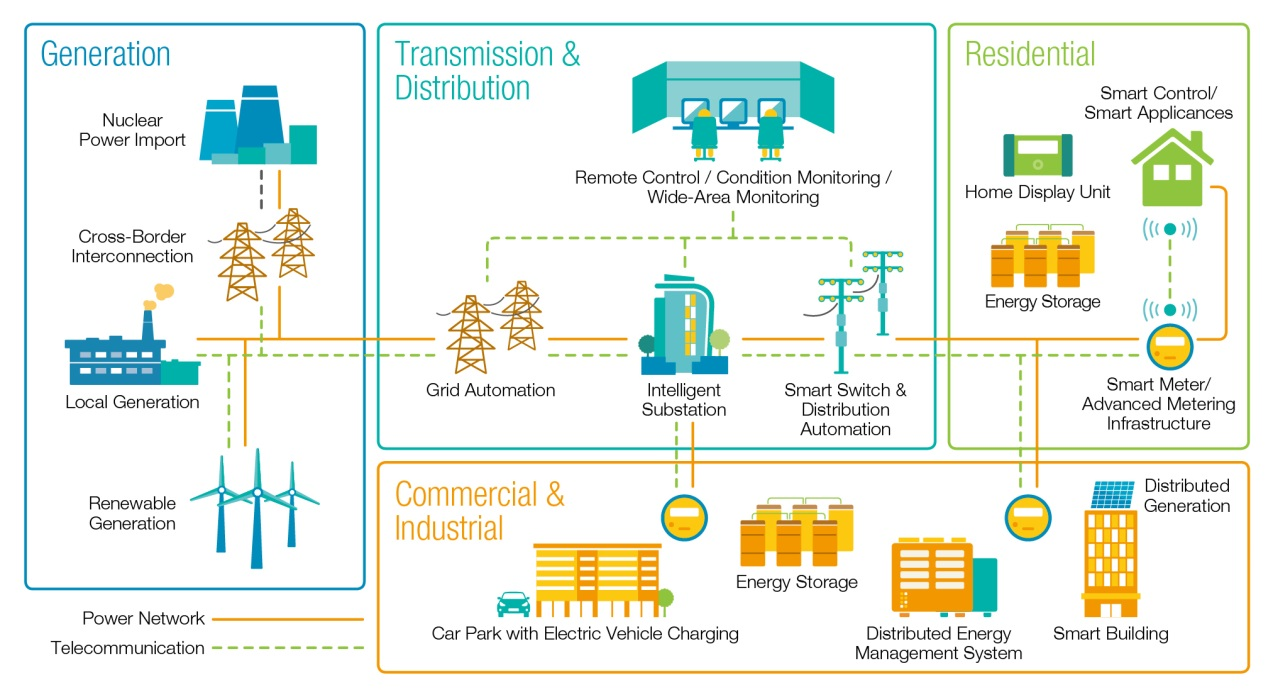
\includegraphics[scale=0.95]{imgs/architecture.jpg}}
\caption{Smart Grid}\label{fig:1}
\end{figure}

\section{Smart Grid Framework}
Le Smart Grid richiedono sia una complessa infrastruttura di comunicazione, che sofisticate tecnologie di comunicazione e computazione. Entrambe consentono la conservazione di parte dell'energia prodotta e l'introduzione di nuovi metodi di gestione della domanda energetica, per adottare politiche di bilanciamento del carico, controllare instabilità energetiche causate dalla natura delle risorse rinnovabili e prevenire la diffusione di fallimenti in cascata nella rete. 
\newline 
La figura \ref{fig:2} riassume le principali tematiche relative alle Smart Grid:
\begin{itemize}
	\item \emph{Energy infrastructure} rappresenta la base fisica ed organizzativa necessaria per la generazione, trasmissione e distribuzione dell'energia;
	\item \emph{Communication infrastructure} è responsabile del trasferimento di informazioni critiche attraverso la rete;
	\item \emph{Information technology} fornisce modelli, analisi, visualizzazioni web e transazioni commerciali;
	\item \emph{Potential applications} offre tecniche di generazione, gestione, automatizzazione e rilevamento per l'intero sistema.
\end{itemize} 

\begin{figure}[h] \centering{
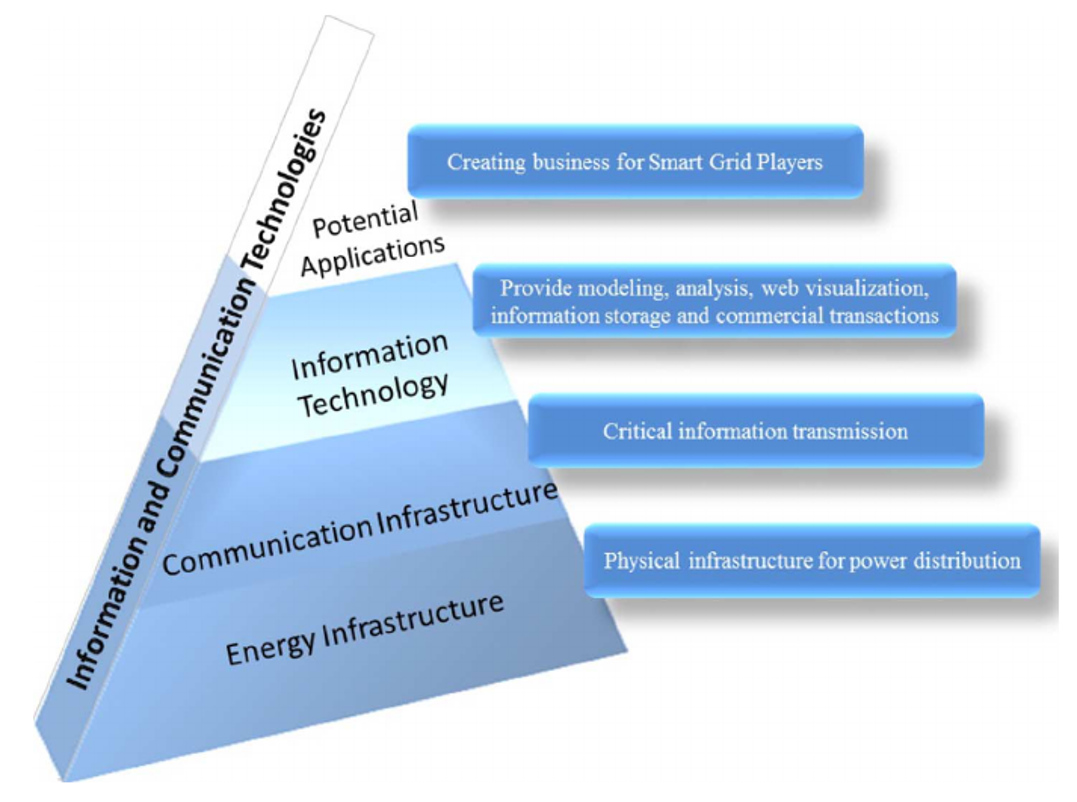
\includegraphics[scale=0.3, natwidth=1003,natheight=490]{imgs/ict.png}}
\caption{Smart Grid framework}\label{fig:2}
\end{figure}

La communication infrastructure svolge un ruolo cruciale, ossia collegare tutte le componenti della rete collezionando informazioni sulle loro condizioni, per scopi di controllo, monitoraggio e manutenzione. Eventuali problemi legati all'energy instrastructure possono essere evitati se corrette operazioni vengono prese con l'aiuto della communication infrastructure. 
\newline 
Differenti tecnologie di comunicazione posso essere usate per diversi scopi e requisiti in base all'applicazione. L'information technology fornisce una piattaforma comune di scambio di informazioni proveniente da differenti attività legate alla Smart Grid, che permette l'integrazione di informazioni da diversi livelli, dando sostegno alla raccolta di diverse informazioni, all'analisi e ad applicazioni avanzate.
\newline
Le tecniche dell'applications layer generalmente mirano a ridurre il consumo energetico dei clienti, cambiando i loro comportamenti di consumo, dotandoli di strumenti di monitoraggio.    
\newline
La figura \ref{fig:3} mostra le componenti della Smart Grid, illustrate dall'energy infrastructure al potentional applications.

\begin{figure}[h] \centering{
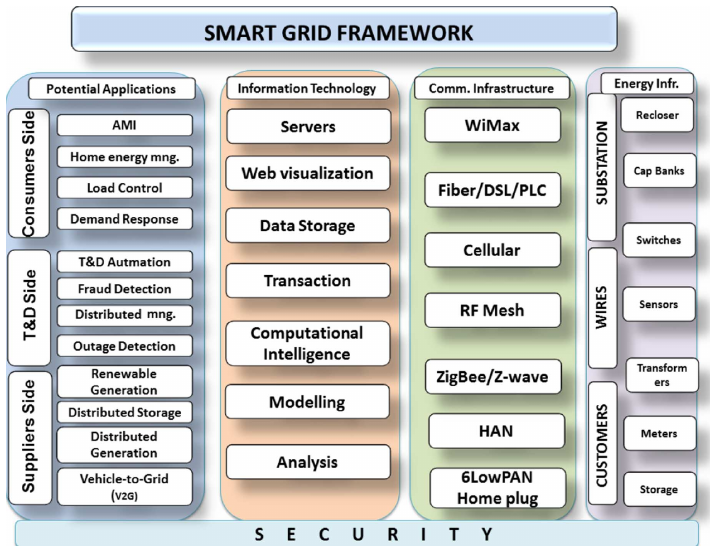
\includegraphics[scale=0.7, natwidth=1003,natheight=490]{imgs/sgframework.png}}
\caption{Smart Grid framework}\label{fig:3}
\end{figure}

%\section{Communication architecture}
\newpage
Il concetto di Smart Grid mira a realizzare un sofisticato sistema, integrando information technology e communication infrastructure all'attuale sistema di alimentazione e il nuovo sistema di generazione distribuito, in modo da sfruttare pienamente l'uso di risorse rinnovabili e di massimizzare l'efficienza energetica. Da una prospettiva leggermente diversa, una Smart Grid può essere considerata come una rete di comunicazione di dati che riesce, grazie al supporto di specifici dispositivi di gestione dell'energia, a far collaborare le diverse componenti della rete in maniera flessibile e senza discontinuità, per un utilizzo efficiente dell'energia.
%\newline
%L'architettura \emph{end-to-end} delle Smart Grid (fig. \ref{fig:4}) fondamentalmente comprendono tre livelli principali:
%\begin{itemize}
%	\item \emph{Application layer}, include applicazioni avanzate fornendo interoperabilità fra di esse; si occupa principalmente della gestione della domanda/risposta, interruzioni, infrastruttura di metering, delle risose ed rilevamento di frodi;
%	\item \emph{Power layer}, comprende i sistemi di generazione, trasmissione e distribuzione, l'integrazione di risorse rinnovabili ed il sistema di comunicazione bidirezionale;  
%	\item \emph{Communication layer}, rappresenta il cuore del sistema fornendo la connettività fra tutte le parti e dispositivi di esso. 
%\end{itemize}     

%\begin{figure}[h] \centering{
%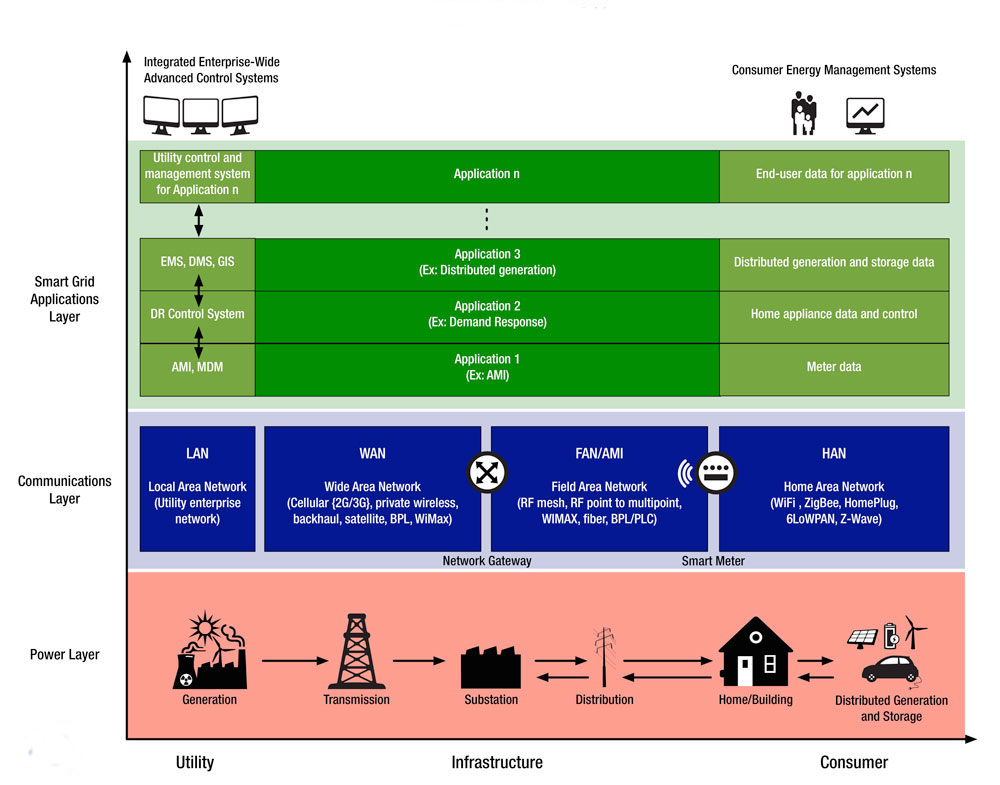
\includegraphics[scale=0.4, natwidth=1003,natheight=490]{imgs/endtoendtax.jpg}}
%\caption{Architettura end-to-end}\label{fig:4}
%\end{figure}

La comunicazione consiste di tre categorie di trasmissione, con relativi standard e protocolli (vedi cap.):
\begin{itemize}
	\item \emph{Wide-area network} (WAN);
	\item \emph{Field-area network} (FAN);
	\item \emph{Home-area network} (HAN).
\end{itemize}

%Il communication layer consiste di tre categorie di trasmissione:
%\begin{itemize}
%	\item \emph{Wide-area network} (WAN);
%	\item \emph{Field-area network} (FAN);
%	\item \emph{Home-area network} (HAN).
%\end{itemize}

\subsection{Wide-area network}
La WAN consente la comunicazione fra le entità che forniscono energia e le substations; deve estendersi su tutte le substation, strutture di distribuzione, generazione energetica e di conservazione dell'energia, per poter essere efficace e scalabile. Essa è rete di comunicazione bidirezionale ad alta larghezza di banda che gestisce le trasmissioni a lunga distanza dei dati con avanzate applicazioni di misurazione e monitoraggio. La comunicazione remota fra le \emph{utility} e gli smart meter è essenziale per lo scambio di importanti informazioni, quali prezzi e tariffe dei clienti. Le reti cellulari, WiMAX e comunicazioni cablate, in particolare comunicazioni basate su fibra ottica e microwave, sono i migliori candidati come tecnlogie per WAN (vedi cap. 4).
\newline
Il sistema di distribuzione agisce da punto di aggregazione fra FAN e WAN, come ad esempio una substation o una torre di comunicazione che colleziona tutte le informazioni prodotte dagli smart meter e le trasferisce alla rete di comunicazione principale. Oltre che da punto di aggregazione tali dispositivi possono fungere da punti di conservazione dell'energia per eventuali interruzioni o guasti.

\subsection{Field-area network}
La FAN può essere descritta come una rete di comunicazione per aree di distribuzione dell'energia e che mette in contatto l'automazione della distribuzione e dispositivi di controllo alle sedi dei consumatori. Essa agisce, quindi, come un intermediario fra le substation e le sedi dei clienti, con nodi intelligenti in grado di raccogliere e controllare i dati da remoto. Tali nodi sono connessi ad un gateway centralizzato, il quale è alimentato costantemente in modo da poter trasmettere i dati raccolti. I canali a bassa larghezza di banda della FAN sono altamente robusti per la trasmissione affidabile di dati. 
\newline 
La scelta delle tecnologie di comunicazione  variano per la FAN in base alle esigenze della Smart Grid: fibra ottica per avere bassa latenza e perfomance di comunicazione superiori, oppure WiMAX se le reti cellulari non riescono a coprire l'area di interesse, ma l'attuale orientamento ricade sull'utilizzo dello standard IEC 61850 (vedi cap. ), il quale fornisce interoperabilità e comunicazione fra i dispositivi elettronici intelligenti.

\subsection{Home-area network}{
Gli smart meter riescono a connettersi alla HAN, in modo tale che i consumatori siano in grado di conoscere l'importo da pagare e gestire il loro consumo ed avere il controllo dei propri elettrodomestici intelligenti, attraverso display presenti in casa e interfacce web. 
\newline 
Le migliori tecnologie di comunicazione per HAN sono ZigBee,Wi-Fi, HomePlug, Z-wave e M-Bus (vedi cap.).
}

\vspace{20pt}\hspace{-17pt}Nelle sezioni successive vengono presentate le tecnologie e le infrastrutture abilitanti di una Smart Grid, a partire dalla generazione e conservazione dell'energia fino ad arrivare alla trasmissione e distribuzione.

\section{Generazione di energia rinnovabile}
Le risorse di energia rinnovabile sono state sviluppate in molti paesi per ridurre l'inquinamento e fornire energia elettrica sostenibile. A differenza delle tradizionali fonti di energia, le quali creano inquinamento, le risorse di energia rinnovabile non esauriscono risorse naturali nel processo di creazione di energia e sono adattabili ovunque, in base alle dimensioni a partire dall'applicazione su una singola casa fino a dimensioni su larga scala.
\newline
Le più comuni risorse di energia rinnovabile sono:
\begin{itemize}
	\item \emph{Sistemi fotovoltaici}, i quali convertono l'energia solare direttamente in elettricità, attraverso pannelli solari esposti al sole. Tali pannelli sono costituiti da celle solari che contengono materiale fotovoltaico, le quali trasmettono elettroni tra diverse bande all'interno del materiale generando differenza di potenziale fra due elettrodi, che consente alla corrente continua di fluire;
	\item \emph{Sistemi per l'energia solare termica}, che convertono energia solare in calore. Esistono tre tipi di raccoglitori in base alla temperatura, da bassa per riscaldare piccoli spazi ad alta per l'utilizzo nella produzione di energia elettrica;
	\item \emph{Vento}, la cui energia viene convertita tramite turbine in elettricità. Il principale aspetto negativo deriva dall'intermittenza del vento, specularmente per i sistemi basati sull'energia solare;
	\item \emph{Biomasse}, ovvero la produzione di elettricità a partire da elementi naturali morti, anche se questa causa inquinamento atmosferico;
	\item \emph{Sistemi che sfruttano la potenza dell'acqua}, sia che essa sia generata artificialmente che naturalmente, grazie alle onde e alle maree.   
\end{itemize} 

 
\section{Conservazione dell'energia}
Il principale problema con l'energia elettrica è che deve essere utilizzata non appena viene generata, o in caso contrario, deve essere convertita in altre forme di energia. Durante i periodi in cui non è richiesta la loro assistenza, sistemi di stoccaggio accumulano energia. Successivamente, l'energia immagazzinata viene inviata nel sistema di alimentazione in determinati periodi di tempo, pertanto
riducendo la richiesta di generazione e assistendo il sistema quando necessario. 
Tali sistemi di conservazione dell'energia vengono sfruttati per diversi scopi:
\begin{itemize}
	\item Mitigare fluttuazioni e perdite momentanee di potenza;
	\item Gestire cambiamenti frequenti di richiesta energetica per garantire stabilità del sistema; 
	\item Sostenere l'intermittenza e a mancanza di controllabilità nella generazione di energia rinnovabile, fornendo l'energia mancante e sottraendo quella in eccesso rispetto alla domanda;
	\item Conservare energia in determinati periodi, ad esempio quando la domanda oppure il prezzo sono bassi e scaricarla quando conviene.
\end{itemize}

Storicamente le centrali idroelettriche sono state le più comuni applicazioni di stoccaggio dell'energia, tuttavia negli ultimi decenni sono state introdotte nuove tecnologie in tale ambito:
\begin{itemize}
	\item Batterie, in grado di immagazzinare energia durante le fasi di carico/scarico;
	\item Pile a combustibile, che permettono di ottenere energia mediante reazioni chimiche senza che avvenga alcun processo di combustione termica, a partire da ossigeno ed idrogeno;
	\item Volani, i quali possono accumulare energia cinetica in masse rotanti e rilasciarla rallentandone la rotazione;
	\item Superconduttori magnetici, capaci  di raccogliere energia in campi magnetici, che vengono creati attraverso il passaggio di corrente continua in super bobine.  
\end{itemize}

\section{Veicoli elettrici}
Le Smart Grid ed i relativi miglioramenti in affidabilità, sostenibilità, sicurezza ed economia della rete elettrica consentono la partecipazione attiva di veicoli alla Smart Grid. I trasporti elettrici sono sempre stati collegati alla tradizionale rete elettrica, in maniera più o meno contigua per alimentare tali veicoli. L'introduzione di meccanismi di conservazione di energia hanno permesso l'uso di veicoli non strettamente legato alla rete.
Sono presenti due tipologie di veicoli elettrici:
\begin{itemize}
	\item \emph{Plug-in}, i quali possono conservare energia grazie a batterie ricaricabili ed utilizzano un motore elettrico per la propulsione;
	\item \emph{Ibridi}, che combinano i motori convenzionali e treni a trazione elettrica per fornire la forza motrice da entrambi i carburanti a combustione interna o energia immagazzinata nelle batterie.  
\end{itemize}     

Esistono due categorie di interazioni energetiche fra i veicoli e la rete elettrica:
\begin{itemize}
	\item \emph{Grid-to-vehicle}, che consiste nella fornitura di energia da parte della rete ai veicoli del tipo plug-in, mediante una presa per la carica;
	\item \emph{Vehicle-to-grid}, in cui il veicolo possiede gli strumenti per fornire energia verso la rete elettrica, considerato come distributore di energia e risorsa di alimentazione nella Smart Grid.
\end{itemize}

Siccome i veicoli non seguono dei meccanismi deterministici e non forniscono una quantità paragonabile a quelle delle classiche tecnologie, rappresentano una sfida per l'integrazione nelle Smart Grid, anche a causa dei costi infrastrutturali. 
%http://www.internationaltransportforum.org/jtrc/discussionpapers/dp201202.pdf
I veicoli elettrici possono essere usati sia come dispositivi di memorizzazione distribuiti, che per fornire l'energia conservata nelle batterie alla rete elettrica o altrettanto alle case. 
Quindi tali mezzi possono fornire aiuto nel bilanciamento del carico, immagazzinando energia la notte e fornendola di giorno alla rete. Essi per il 95\% del tempo sono parcheggiati, fornendo così l'opportunità di usare la loro energia, in modo da ridurre costi del sistema elettrico.


\section{Microgrid}
Una microgrid è un sistema energetico locale, che offre integrazione di risorse energetiche    distribuite con le risorse che usufruiscono di tale energia, il quale può operare sia con la Smart Grid che in maniera isolata per fornire un livello personalizzato di affidabilità e resilienza. 
Fra i principali vantaggi delle microgrid:
\begin{itemize}
	\item Costituiscono un passo avanti economico ed efficiente per portare elettricità nelle zone rurali;
	\item Offrono una soluzione per alleviare la pressione dovuta alla saturazione della rete in determinate aree, senza grandi sforzi economici;
	\item Isolano determinati e sensibili consumatori, come basi militari e ospedali;
	\item Possono contribuire nella gestione della domanda energetica delle risorse rinnovabili;
	\item Sono in grado di contribuire nella conservazione dell'energia, nel miglioramento della stabilità e affidabilità delle rete elettrica.	  
\end{itemize}
Il maggior numero di tipi di microgrid sono istituzionali (ospedali, universPMUità o zone militari), seguiti da commerciali (fattorie, server farm, centri commerciali) ed infine di comunità (gruppi di case o appartamenti).  
Una microgrid è formata da componenti disponibili sul mercato, quali:
\begin{itemize}
	\item \emph{Sensori}, determinano quali criteria adottare, se di isolamento o connessione alla rete elettrica;
	\item \emph{Switch e contatori intelligenti}, consentono rapide riconfigurazioni e monitoraggio in tempo reale;
	\item \emph{Generatori di energia} e \emph{dispositivi per la conservazione dell'energia}.   
\end{itemize}

\section{Smart substation}
Una substation elettrica è un punto di riferimento dei sistemi di generazione, trasmissione e distribuzione, dove il voltaggio viene trasformato da alto a basso e oppure viceversa utilizzando trasformatori. La corrente elettrica scorre attraverso diverse substation fra impianti di generazioni e clienti. Ci sono diversi tipi di substation: trasmissione, distribuzione, raccolta, smistamento. Le funzioni generali includono:
\begin{itemize}
	\item Trasformazione del voltaggio;
	\item Punto di connessione delle linee energetiche di trasmissione e distribuzione;
	\item Centro di smistamento delle configurazioni dei sistemi di trasmissione e distribuzione;
	\item Zona di monitoraggio per il centro di controllo;
	\item Protezione per gli apparecchi e linee elettriche;
	\item Comunicazione con le altre substation e i centri di controllo. 
\end{itemize} 
Le substation sono le fonti dei dati in tempo reale fondamentali per il funzionamento efficiente e sicuro della rete. I dati reali sono valori istantanei dei sistemi di alimentazione e vengono usati per la protezione, monitoraggio e controllo delle apparecchiature di tali sistemi. Vi è anche una ricchezza di dati non in tempo reale disponibile dalle apparecchiature, generalmente segnalazioni, che aiuta a rendere il funzionamento e la gestione delle attività di sistema più efficiente e affidabile.
\newline
%0deec5301d9ee1c662000000.pdf
Il concetto di smart substation, che si basa sulle tecnologie automatiche delle substation, consente monitoraggio più affidabile ed efficiente, funzionamento, controllo, protezione e manutenzione delle attrezzature e apparecchiature installate nelle sottostazioni. Per raggiungere questi obiettivi, le caratteristiche principali delle smart substation sono:
\begin{itemize}
	\item \emph{Digitalizzazione}, un'unica e compatibile piattaforma per la rilevazione, misurazione, comunicazione, controllo, protezione e manutenzione, che comunica con i centri di controllo;
	\item \emph{Autonomia} e {coordinazione}, il funzionamento non dipende da altre substation o centri di controllo, ma possono comunicare per incrementare l'efficienza e la stabilità della trasmissione elettrica. Anche all'interno stesso della smart substation, i singoli componenti devono essere autonomi;
	\item \emph{Autoconfigurazione}, abilità nel configurarsi autonomamente in maniera dinamica, per ristabilirsi da attacchi, blackout, fallimenti delle componenti oppure disastri naturali.   
\end{itemize}   

Le funzioni essenziali di una smart substation comprendono:
\begin{itemize}
	\item \emph{Rilevamento e misurazione smart}, tutti i segnali misurati vengono etichettati con alta accuratezza grazie a sistemi di posizionamento (GPS);
	\item \emph{Comunicazione}, ogni smart substation ha un LAN ad alta velocità, che lega tutte le unità di misuramento e le applicazioni locali insieme, ed interfacce di connessione per diversi tipi di comunicazione. Il protocollo di comunicazione di una smart grid dovrebbe essere \emph{open} e standardizzato ed una buona opzione è lo standard \emph{IEC 61850} (vedi ..);
	\item \emph{Controllo autonomo}, controllori decentralizzati vengono usati per l'auto-ripristino, per intraprendere azioni correttive o di previsione e ottimizzazione. I tradizionali controller \emph{volt/Var} basati sulle informazioni di misurazione locali(vedi ...) vengono coordinati da centri di controllo. Condizioni di instabilità valutati più velocemente dalle informazioni dei\emph{PMU} (vedi ..) [45], [46];
	\item \emph{Gestione e visualizzazione dei dati}, applicazioni decentralizzate richiedono un appropriato sistema di gestione di dati distribuito, il quale gestisca e condivida i dati con le altre substation e che comunichi con centri di controllo. Tutti i dati dai PMU, i ritardi, resoconti di fallimenti ed ecc. devono essere visualizzati in tempo reale per fornire una chiara visione dello stato della substation. 
\end{itemize}
 
\subsection{IED}
\emph{Intelligent Electronic Devices} (IED) sono dei dispositivi basati su microprocessore, che hanno la capacità di scambiare dati e segnali di controllo con altri dispositivi, come altri IED, misuratori elettrici, controller e SCADA, mediante canali di comunicazione. Gli IED svolgono funzioni di protezione, monitoraggio, controllo e acquisizione di dati nelle stazioni di generazione, substation ed alimentatori. Essi sono largamente usati nelle substation per diversi scopi e vengono utilizzati anche separatamente per ottenere funzioni individuali. Gli IED sono una componente chiave di integrazione e di automazione delle substation, le quali comportano l'integrazione delle funzioni di protezione, controllo e acquisizione dei dati in modo da ridurre i costi operativi e di capitale, eliminando apparecchiature ridondanti e riducendo al minimo l'intervento umano. Tali dispositivi sono totalmente compatibili con lo standard IEC  61850 (vedi ..), hanno dimensioni ridotte e combinano varie funzioni in un'unica struttura robusta, consentendo una riduzione delle dimensioni dell'intero sistema, un aumento dell'efficienza e di robustezza, fornendo soluzioni estendibili basati su tecnologie di comunicazione tradizionali. 

\subsection{Sensori}
La principale funzione dei sensori è quella di raccogliere i dati provenienti da apparecchiature di alimentazione e portarle alle componenti delle substation, in particolare trasformatori, interruttori e linee elettriche. Con l'introduzione delle tecnologie digitali e ottiche, nuovi sensori sono diventati disponibili per acquisire diversi tipi di informazioni relative a determinate risorse. L'apparato analogico basato su fili di rame può essere sostituito da fibra ottica per misurazione e monitoraggio.
\newline
I vantaggi più importanti di tali sensori sono:
\begin{itemize}
	\item Maggiore precisione;
	\item Nessuna saturazione;
	\item Dimensioni e peso ridotti;
	\item Sicuri e non dannosi per l'ambiente;
	\item Prestazioni e larghezza di banda più elevate;
	\item Bassa manutenzione.
\end{itemize}


\subsection{SCADA}
\emph{Supervisory Control And Data Acquisition} (SCADA) si riferisce a un sistema o una combinazione di sistemi che raccoglie i dati provenienti da vari sensori in un impianto o in altre posizioni remote e che invia questi dati ad un elaboratore centrale, che poi gestisce e controlla i dati e controlla da remoto i dispositivi nel campo. SCADA è un termine che viene utilizzato ampiamente per rappresentare soluzioni di controllo e di gestione in una vasta gamma di settori. Il settore elettrico ha un insieme specifico di requisiti che si applicavano ai sistemi SCADA. Lo scopo principale di un sistema SCADA elettrico è quello di acquisire dati in tempo reale provenienti dai dispositivi situati nelle centrali elettriche, sottostazioni di trasmissione e di distribuzione, alimentatori per distribuzione, ecc, fornire il controllo delle apparecchiature e presentare le informazioni al personale operativo.  
\newline
Sistemi SCADA sono globalmente accettati come mezzo di monitoraggio e controllo di sistemi di alimentazione elettrica, in particolare sistemi di generazione e trasmissione in tempo reale. \emph{RTU} (Remote Terminal Units) vengono utilizzati per raccogliere i dati analogici e lo stato di telemetria dai dispositivi, e di trasmettere comandi di controllo a tali dispositivi. Installato in una posizione centrale, come ad esempio il centro di controllo, tali sistemi includono apparecchiature di acquisizione dati, interfacce grafiche per gli operatori, applicazioni che agiscono sui dati e altri componenti. 
\newline
Tipicamente apparecchiature di controllo di acquisizione dati comprendono almeno una \emph{master statuion} (vedi ..), uno o più RTU e un sistema di comunicazione. La master station di solito è collocata al centro di controllo dell'energia, mentre gli RTU sono installati nelle centrali elettriche, substation di trasmissione e distribuzione e attrezzature di alimentazione.

\section{Sistemi di trasmissione}

\subsection{Sistemi di gestione dell'energia}
\subsection{FACTS}
\subsection{HVDC}
\subsection{WAMPAC}


\section{Sistemi di distribuzione}

\subsection{Sistemi di gestione della distribuzione}
\subsubsection{distribution SCADA}
\subsection{Volt/VAr control}


%
%\subsection{smart substation} 3.3 , 3.3.8 role
%IED, sensor, scada, RTU, 
%
%\subsection{energy storage}
%veicoli, microgrid (3.2.4)
%
%\subsection{generazione di energia da risorse rinnovabili}
%
%\subsection{trasmission systems} 3.4 (pag.154) role 209
%facts hdvc 3.4.2 (pag.168), WAMPC 3.4.3 (pag.187) 202 role
%
%\subsection{distribution systems} 3.5 pag.211
%distribution scada, Fault Detection, Isolation, and Service Restoration 244, componenti, outage management
%
%\subsection{communication systems} 265
%ami, 
%
%\subsection{monitoring and diagnostics}
%
%\subsection{SMART METERS AND ADVANCED METERING INFRASTRUCTURE}
%
%vedere anche 3.4.1.4 



% http://ieeexplore.ieee.org/stamp/stamp.jsp?tp=&arnumber=6298960 

%http://www.smartgridinformation.info/pdf/5264_doc_1.pdf

% http://www.cs.nmsu.edu/~misra/papers/SmartGridSurvey.pdf


%libri 

